% arara: pdflatex: {synctex: yes, action: nonstopmode, options: "-file-line-error-style"}
% arara: bibtex
% arara: pdflatex: {synctex: yes, action: nonstopmode, options: "-file-line-error-style"}
% arara: pdflatex: {synctex: yes, action: nonstopmode, options: "-file-line-error-style"}

\documentclass{article}
\usepackage{cite}
\usepackage{url}
\usepackage[bottom]{footmisc}
\usepackage{pdfpages}
\usepackage{graphicx}
\usepackage{natbib}
\usepackage{listings}
\usepackage{color}
\usepackage{amsmath}
\usepackage{framed}
\lstdefinestyle{customc++}{
	belowcaptionskip=1\baselineskip,
	breaklines=true,
	numbers=left,
	frame=single,
	xleftmargin=\parindent,
	language=C++,
	captionpos=b,           % sets the caption-position to bottom
	showstringspaces=false,
	basicstyle=\footnotesize\ttfamily,
	keywordstyle=\bfseries\color{green!40!black},
	commentstyle=\itshape\color{purple!40!black},
	identifierstyle=\color{blue},
	stringstyle=\color{orange},
}
\title{Embedded Real Time Systems - Project}
\author{Daniel Ejnar Larsen and Christian M. Lillelund}
\date{\today}
\begin{document}
\maketitle
\begin{abstract}
	In this report, a genetic optimization algorithm is modeled in SystemC, then verified and accelerated in an FPGA using Vivado's HLS tool to find if this kind of global search algorithm benefits from hardware acceleration. The results of comparing the algorithm evaluated on a standard general-purpose processor with the hardware accelerated version in terms of performance, energy usage and space are presented.
\end{abstract}


\section{Introduction}
Optimizing traditional software algorithms using hardware acceleration, like field-programmable gate array (FPGA's), is an active area of research and development due the potential decrease in latency and increase in throughput. With high-level synthesis (HLS) we refer to a process where the actual logical description of system functionality is described in a abstract modeling language, like the C-based SystemC, before being synthesized to a hardware description language like VHDL or Verilog and then executed in an FPGA on a system-on-a-chip (SoC) board. This approach makes use of a hardware and software co-design methodology to create a computational specification model in software used to generate a design that can be deployed to hardware. This brings a shorter design time, a decrease in time to market and a opportunity to evaluate many potential design options. In this report, we use HLS to describe, design and simulate a genetic optimization algorithm that finds the global minimum on the Xilinx ZyBo platform using Vivado's high-level synthesis (HLS) tool. The actual algorithm is modeled in SystemC, verified and then accelerated in an FPGA as an intellectual property (IP) core. To benchmark the algorithm, we use the two-dimensional non-convex Rosenbrock function\cite{Shang2006} given a set of user-set parameters, where the minimum resides in a parabolic-shaped valley.

All source code developed through this project is available in the zip file \textit{src.zip} with code for the two SystemC models (in folders GenerationGenerator and RosenborckSimulator) and the C++ user application (the folder userapp).

\section{Methodology}

\begin{framed}
1. Define a methodology using SysML/UML diagrams for the development of your system. Specify SysML/UML diagrams that need to be made in the different phases of the project. Make a short description of each design phases and the SysML/UML diagrams and profiles you decide to use in the methodology. Remember to use references to the papers you have use as inspiration for your work. Decide on an UML2 tool.
\end{framed}


The working methodology for this report will be combination of SysML \cite{sysml}(OMG 04-2006) and UML \cite{uml} (OMG 08-2006). With SysML, the non-software parts of the system can be described, e.g. the synthesized mapping onto the hardware or other register-transfer level (RTL) models. UML on the other hand provides a logical and discrete description of software classes or their interaction. As we are modeling a solution based on hardware and software co-design, both methodologies are applicable and will be described in section \ref{sec:archdesign}, architecture and design. The diagrams and models will be derived from a set of requirements put forward in section \ref{sec:req}, requirements. To quickly review the identified diagrams for this report:

\begin{itemize}
	\item Internal block diagram (IBD): To model block-specific inputs and outputs of the algorithm IP block.
	\item State machine diagram: To model the different state of the system, their transitions and guards.
	\item Activity diagram. To show the sequence of actions of the application and which activities it goes through. These are useful to get an overall idea of the use case.
	\item Class diagrams. Depicts the logical software classes, their dependencies and associations.
\end{itemize}

The analysis, design, development and validation phases follow the model-based co-design with UML/SysML described in X. This holistic process takes a starting point in the requirements, derives an architecture and design of the system, then proceeds to an implementation phase where high-level source code is designed, simulated and synthesized to a hardware description language (HDL). It concludes by conducting an entire system validation.


\section{Requirements}\label{sec:req}

\begin{framed}
2. Write a requirement specification with functional and non-functional requirements especially with focus on performance like throughput and latency. The functional requirements can be described in terms of use cases.
\end{framed}

The following functional and non-functional are stated for this report as they make up the system and architectural design:

\begin{itemize}
\item The system must be able to generate a new generation using the genetic algorithm.
\item The system must perform a simulation to evaluate the fitness of the generation using the Rosenbrock function.
\item The system should be able to generate a new generation as fast as possible.
\item The system should be able to perform a simulation of a generation as fast as possible.
\item The simulation should have user configurable parameters $a$ and $b$.
\item The user should be able to extract the generation and its fitness from the system.
\end{itemize}

The functional non-functional requirements are stated in the form of a use case.
This use case is described in table \ref{tab:usecase}. Here it can be seen, that the flow, seen from the user perspective, is rather simple. The user basically asks for a specific Rosenbrock function to be optimized, and gets a chromosome, that optimizes it.

\begin{table}[htbp]
\caption{Basic use case for the system.} \label{tab:usecase}
\begin{tabular}{l|l}
\hline
\textbf{Goal}          & \begin{tabular}[l]{@{}l@{}}The user has gotten an optimized\\ chromosome\end{tabular}                                                                                                                                                                                                                                                                                                   \\ \hline
\textbf{Initializer}   & The user                                                                                                                                                                                                                                                                                                                                                                                \\ \hline
\textbf{Actor}         & The user                                                                                                                                                                                                                                                                                                                                                                                \\ \hline
\textbf{Prerequisits}  & \begin{tabular}[l]{@{}l@{}}The system is turned on and has\\ done its initialization.\end{tabular}                                                                                                                                                                                                                                                                                      \\ \hline
\textbf{Result}        & \begin{tabular}[l]{@{}l@{}}The user gets an optimized\\ chromosome\end{tabular}                                                                                                                                                                                                                                                                                                         \\ \hline
\textbf{Main Scenario} & \multicolumn{1}{l}{\begin{tabular}[c]{@{}l@{}}1. The user runs the setup\\ 2. The user enters the wanted setup parameters.\\ 3. The user starts an optimization.\\ 4. The system performs the optimization.\\ 5. The system generates a new generation.\\ 6. Repeat from step 4 until stopping criterion is met.\\ 7. The user extracts the final chromosome and fitness.\end{tabular}}
\end{tabular}
\end{table}
 
 

\section{Theory}\label{sec:theory}

This section will briefly explain the theory behind the genetic algorithm. It is defined as a randomized, population based global search algorithm that tries to find global maxima or minima of a certain function $f(x)$, in our case the Rosenbrock function: $$f(x,y) = (a-x)^2+b(y-x^2)^2$$ where $a$ and $b$ are parameters that define the function and $x$ and $y$ its coefficients. We start with an initial population $P_{(0)}$ in which $x$ and $y$ are given as chromosomes (binary strings) of a certain size and evaluate the objective function (the Rosenbrock function\cite{Shang2006}) at points in $P_{(0)}$ to get a fitness $F_{i}$ for each chromosome. The fitness represent a chromosome's score on the function, as a high value means we are close to either a global optimum or minimum. We save the fitness as the best-so-far chromosome and continue to create population $P_{(1)}$ from $P_{(0)}$ using the chromosomes with the best fitness so far, evaluate its fitness and so forth in an iterative manner. Given iteration $k=0$ and a initial population $P_{(0)}$, the algorithm can be defined as\cite{Chong2013}:

\begin{enumerate}
	\item Evaluate $P_{(k)}$. If stopping criterion is met, then stop.
	\item Select $M_{(k)}$ from $P_{(k)}$ as the mating pool.
	\item Create new chromosomes from mating pool $M_{(k)}$ by crossover and mutation.
	\item Increase $k$ by one and start over.
\end{enumerate}

An interesting aspect is the crossover and mutation part, where we create new chromosomes (children) from binary strings (parents) with the best fitness of a population and mutate them afterwards. Figure \ref{fig:geneticalgocrossover} shows an example of a crossing, where the bit set of two parents are mixed at crossing sites to form two children. The crossing sites are chosen at random. Given two bit strings, e.g. $0000$ and $1111$, the mutation shown in figure \ref{fig:geneticalgocrossover} would form two children $1001$ and $0110$. What follows is a mutation operation, where we flip bits in the children's bit string with a given probability $p_{m}$, usually a small value ($p_{m} < 0.01$), so only few chromosomes will be mutated. The idea behind these random crossings and mutations is that we seek a global maximum or minimum of our function $f(x)$ anywhere in the search space by avoiding getting stuck in local maximums or minimums, as is the case with gradient search methods. The particle swarm algorithm (PSO) shares similar attributes with genetic optimization.

\begin{figure}[h]
	\centering
	\fbox{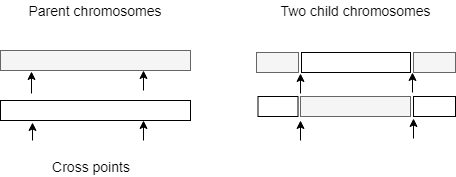
\includegraphics[width=0.7\linewidth]{theory/GeneticAlgoCrossover.png}}
	\caption{An example of two parent chromosomes being crossed to create two children.}
	\label{fig:geneticalgocrossover}
\end{figure}




\section{Architecture and Design}\label{sec:archdesign}

\subsection{Architecture}
\begin{framed}
3. Use your design methodology found in 1. to describe a SysML/UML model of your system in terms of structure and behavior. Make a suggestion for alternative HW/SW architectures. Decide on which parts of the functionality should be mapped to hardware components and software processes.
\end{framed}

The overall structure of the system can be seen in the BDD in figure \ref{fig:bdd}. Here it can be seen, that the system should consist of three parts: \emph{User Interface}, \emph{Generation Generator}, and \emph{Simulator}. Each of the blocks has its own responsibility. \emph{User Interface} is responsible for getting the input from and to the user, e.g. the start generation and the final generation and fitness. \emph{Generation Generator} is responsible for generating the new generation using the genetic algorithm. \emph{Simulator} is responsible for calculating the fintness, i.e. the Rosenbrock function.

\begin{figure}[htbp]
\begin{centering}
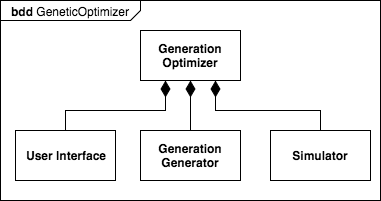
\includegraphics[width=0.7\linewidth]{../diagrams/bdd.png}
\caption{BDD of the system.}
\label{fig:bdd}
\end{centering}
\end{figure}





NOTE: waits in rosenbrock to reduce resources used


\subsection{Design}

\begin{framed}
4. Design the software and apply design patterns that are suitable for your project, and motivate the choice of the used patterns. Use the Two-Part Architecture Model if relevant for the problem. Use the abstract OS package for the ZYBO board
\end{framed}

\section{Modeling in SystemC}\label{sec:modelsystemc}

This section explains how parts of the genetic algorithm has been modeled in SystemC and exported to hardware using HLS with Vivado. As seen in figure \ref{fig:allocation}, two components from the design can be mapped to hardware, so we build a SystemC model for each and evaluated it in the results, see section \ref{sec:results}. Both designs are made at an algorithmic abstraction level. This means that the communication between isolated components is abstracted away, i.e. external stimuli is simply modeled as a signal of some type and outputs are registered in a trace file. However the model is clocked, meaning we have a mean of synchronization, so the modules are approximately timed. The two different modules will be described in the following subsections.

\subsection{GenerationGenerator}
The \textbf{GenerationGenerator} is responsible for generating a new generation of chromosomes using the generative algorithm described previously. Using SystemC, the module consists of two SC\_CTREAD's, as it can be seen in listing \ref{lst:generationgenerator_h}. The module has a number of input and output signals, as most are self-explanatory, we will briefly review them here. The two parent inputs for generation $P_{(k)}$ stem from $P_{(k-1)}$, similar the two children of $P_{(k)}$ are parents of $P_{(k+1)}$. A chromosome has length of 64, where 32 bits are reserved for the $x$ coefficient and 32 for the $y$ coefficient of the Rosenbrock function. Mutation probability is a hyper parameter set as stimuli or from the user side. The two indexes for random numbers are used to keep track of the next random number accessed by $trueRandom()$ and created continually by $produceRandom()$.  \emph{CHR\_WIDTH} is the chromosome width.

\begin{lstlisting}[style=customc++, caption={GenerationGenerator.h},label={lst:generationgenerator_h}]
#include <systemc.h>

#define CHR_WIDTH 64
#define RANDOM_WIDTH 24
SC_MODULE(GenerationGenerator) {
  sc_in<bool> clk;
  sc_in<bool> reset;
  sc_in<bool> startGenerating;
  sc_out<bool> generatingDone;
  sc_in<sc_uint<CHR_WIDTH>> generation_parent1;
  sc_in<sc_uint<CHR_WIDTH>> generation_parent2;
  sc_out<sc_uint<CHR_WIDTH>> generation_child1;
  sc_out<sc_uint<CHR_WIDTH>> generation_child2;
  sc_in<sc_uint<RANDOM_WIDTH>> mutation_probability;
  sc_in<sc_uint<RANDOM_WIDTH>> random;
  sc_uint<RANDOM_WIDTH> randomNumberIndex;
  sc_uint<RANDOM_WIDTH> trueRandomIndex;;
  sc_uint<RANDOM_WIDTH> randomNumbers[GENERATION_SIZE * 16];

  void consumeRandom(void);
  sc_uint<RANDOM_WIDTH> produceRandom(void);
  void generateGeneration(void);
  
  SC_CTOR(GenerationGenerator) {
    randomNumberIndex = 0;
    trueRandomIndex = 0;
    SC_CTHREAD(generateGeneration, clk.pos());
    reset_signal_is(reset,false);
    SC_CTHREAD(consumeRandom, clk.pos());
    reset_signal_is(reset,false);
  }
};
\end{lstlisting}

The modeling of \textbf{GenerationGenerator} is done in SystemC. Listing \ref{lst:trueandproducerandom_cpp} shows the two functions that produce and return a random number, listing \ref{lst:generationgeneratorpragma_cpp} shows pragmas for the $generateGeneration()$ function and listing \ref{lst:generationgenerator_cpp} shows the actual implementation of the function $generateGeneration()$. Function $produceRandom()$ takes the random numbers from the input and saves them in a circular buffer. These random numbers were supposed to come from a loose audio channel, i.e. true random noise, but due to time constraints it was implemented using pseudo random numbers with the C++ $rand()$ function. Function $trueRandom()$ is used to get the random numbers when needed from the circular buffer.

\begin{lstlisting}[style=customc++,caption=The two methods for producing and accessing a random number., label={lst:trueandproducerandom_cpp}]
void GenerationGenerator::produceRandom(void) {
#pragma HLS resource core=AXI4LiteS metadata="-bus_bundle slv0" variable=random
	sc_uint<RANDOM_WIDTH> tmpRnd;
	while(true){
		randomNumbers[randomNumberIndex] = random.read();
		if(randomNumberIndex == RANDOM_WIDTH-1) {
			randomNumberIndex = 0;
		} else {
			randomNumberIndex = randomNumberIndex + 1;
		}
	}
}

sc_uint<RANDOM_WIDTH> GenerationGenerator::trueRandom(void) {
	sc_uint<RANDOM_WIDTH> randomNumber = randomNumbers[trueRandomIndex];
	if (trueRandomIndex == RANDOM_WIDTH - 1) {
		trueRandomIndex = 0; }
	else {
		trueRandomIndex = trueRandomIndex + 1;
	}
	return randomNumber;
}
\end{lstlisting}  

All signals are made available through the AXILite interface by the use of pragmas, e.g. \#pragma HLS resource core=AXI4LiteS metadata="-bus\_bundle slv0" variable=generation\_parent1, also seen in listing \ref{lst:generationgeneratorpragma_cpp}.

\begin{lstlisting}[style=customc++,caption=Pragmas defined for the GenerationGenerator function generateGeneration().,label={lst:generationgeneratorpragma_cpp}]
void GenerationGenerator::generateGeneration(void) {
  #pragma HLS resource core=AXI4LiteS metadata="-bus_bundle slv0" variable=generation_parent1
  #pragma HLS resource core=AXI4LiteS metadata="-bus_bundle slv0" variable=generation_parent2
  #pragma HLS resource core=AXI4LiteS metadata="-bus_bundle slv0" variable=generation_child1
  #pragma HLS resource core=AXI4LiteS metadata="-bus_bundle slv0" variable=generation_child2
  #pragma HLS resource core=AXI4LiteS metadata="-bus_bundle slv0" variable=generation_parent1
  #pragma HLS resource core=AXI4LiteS metadata="-bus_bundle slv0" variable=mutation_probability
  #pragma HLS resource core=AXI4LiteS metadata="-bus_bundle slv0" variable=startGenerating
  #pragma HLS resource core=AXI4LiteS metadata="-bus_bundle slv0" variable=generatingDone

  ...
\end{lstlisting}  

The $generateGeneration()$ functions contains most the logic related to generating generations. It basically implements the generative algorithm as described in theory with two random crossover points. This is done using bit masks which are AND'ed onto the parent chromosomes in the mating pool to produce new children. Each child are then mutated by a stochastic process, where a single bit in the chromosome is flipped if a given random number is lower than a scaled probability of the mutation likelihood.

\begin{lstlisting}[style=customc++,caption={GenerationGenerator.cpp},label={lst:generationgenerator_cpp}]
void GenerationGenerator::generateGeneration(void) { 
  while(true) {
    wait();	
    while (startGenerating->read() == false) { wait(); }
    generatingDone->write(false);
    sc_uint<CHR_WIDTH> parent1 = generation_parent1->read();
    sc_uint<CHR_WIDTH> parent2 = generation_parent2->read();

    // Make crossover points
    sc_uint<CHR_WIDTH> notZero = pow(2, CHR_WIDTH) - 1;
    sc_uint<RANDOM_WIDTH> point1 = trueRandom();
    sc_uint<RANDOM_WIDTH> point2 = trueRandom();

	point1 = (point1 * (CHR_WIDTH - 1)) >> RANDOM_WIDTH;
	point2 = (point2 * (CHR_WIDTH - 1)) >> RANDOM_WIDTH;
	
    // Sort high and low points
    sc_uint<RANDOM_WIDTH> highNum;
    sc_uint<RANDOM_WIDTH> lowNum;
    if(point1 > point2) {
      highNum = point1;  lowNum = point2;
    } else {
      highNum = point2; lowNum = point1;
    }
  
    sc_uint<CHR_WIDTH> bitMask1 = notZero >> lowNum & ~notZero >> highNum;
    sc_uint<CHR_WIDTH> bitMask2 = ~bitMask1;
    sc_uint<CHR_WIDTH> child1 = (parent1 & bitMask1) + (bitMask2 & parent2);
    sc_uint<CHR_WIDTH> child2 = (parent1 & bitMask2) + (bitMask1 & parent2);

    sc_uint<RANDOM_WIDTH> randomMutationProb = mutation_probability.read();

    // Mutating children
    for (int j = 0; j < CHR_WIDTH; j++) {
      if (trueRandom() < randomMutationProb) {
        child1 ^= (1 << j);
      }
      if (trueRandom() < randomMutationProb) {
      	child2 ^= (1 << j);
      }
    }
    
    generation_child1->write(child1);
    generation_child2->write(child2);
    generatingDone->write(true);
  }
}
\end{lstlisting}

The \textbf{GenerationGenerator} module is tested in a test bench that stimulates function calls to it. It simply wires the stimulation and the module together and makes a .VCD trace file with all the signals over the period of the application execution cycle, which is included in the results. Source code for the test bench can be found in the attached code (GenerationGenerator/main.cpp)

\subsection{Simulator}
The simulator (also called the RosenbrockSimulator in code) simulates the Rosenbrock function. The definition in SystemC can be found in listing \ref{lst:rosenbrock_h}. Function $simulateRosenbrock()$ evaluates the fitness of a chromosome from $P_{(k)}$. It should be noted that coefficients $a$ and $b$ are uint32 type signals but handled as floats in the implementation, as we were not able to successfully pass floats over the signals in SystemC. To obtain a floating value for the calculation, we simply make a type conversion using pointers. Signal \emph{chromosome\_in} is passed as input from the user side. The module outputs the actual fitness of the chromosome.

\begin{lstlisting}[style=customc++,caption={RosenbrockSimulator.h},label={lst:rosenbrock_h}]
#include <systemc.h>

#define CHROMOSOME_WIDTH 64
SC_MODULE(RosenbrockSimulator) {
  sc_in<bool> clk;
  sc_in<bool> reset;
  sc_in<bool> startSimulation;
  sc_out<bool> simulationDone;
  sc_in<sc_uint<32>> a; //actually float
  sc_in<sc_uint<32>> b; //actually float
  sc_in<sc_uint<CHR_WIDTH>> chromosome_in;
  sc_out<sc_uint<32>> fitness; //actually float

  void simulateRosenbrock(void);

  SC_CTOR(RosenbrockSimulator) {
    SC_CTHREAD(simulateRosenbrock, clk.pos());
    reset_signal_is(reset,false);
  }
};
\end{lstlisting}

The function implementation of $simulateRosenbrock()$ is viewed in listing \ref{lst:rosenbrock_cpp}. This is done using floats as an experiment, however it is not the most efficient thing to use resource-wise, but brings a better accuracy of the fitness value than fixed-point would, as the function we are looking to minimize is non-convex, i.e. multiple locally optimal points. As seen later in results in section \ref{sec:results}, we discovered there was not enough space for the module on the FPGA in terms of DSP's and LUT's. This could have been made differently by using another floating point encoding which could allow for the use of fixed point arithmetics and interpret it as floats later. $uint32ToFloat()$ is a utility function that converts a unsigned integer number to a float by a simple pointer type cast.

\begin{lstlisting}[style=customc++,caption={RosenbrockSimulator.cpp},label={lst:rosenbrock_cpp}]
#include "RosenbrockSimulator.h"
#include <string.h>
#include <math.h>
#include "ieee754float.h"

void RosenbrockSimulator::simulateRosenbrock(){
  while (true) {
    sc_uint<CHR_WIDTH> notZero = pow(2, CHR_WIDTH) - 1;
    while(startSimulation->read()==false){ wait(); }
    simulationDone->write(false);
    
    sc_uint<CHR_WIDTH> tmpChromosome = chromosome_in->read();
    sc_uint<CHR_WIDTH/2 > x = 0, y = 0;
    x = tmpChromosome >> ( CHR_WIDTH >> 1 );
    y = tmpChromosome;
    
    // Convert coefficients to floats
    float x_float = uint32ToFloat((uint32_t)x);
   	float y_float = uint32ToFloat((uint32_t)y);
   	
   	// Convert parameters to floats
   	float a_local = uint32ToFloat(a->read());
   	float b_local = uint32ToFloat(b->read());
   
   	// Evaluate Rosenbrock function with given data
    uint32_t result = pow((a_local-x_float),2)+
    		b_local*pow((y_double-pow(x_float,2)),2);
    fitness->write(result);
    simulationDone->write(true);
  }
}
\end{lstlisting}

This module is tested using a test bench in the Vivado HLS IDE. This test bench can be found in the attached code (RosenbrockSimulator/main.cpp).

\subsection{Hardware Block Design}

Lastly we view the Vivado hardware block design in figure \ref{fig:vivadodesign}. This is where we import and connect the different IP cores.
We have imported the \textbf{GenerationGenerator} RTL IP core from Vivado HLS after synthesis and wired it with an AXI interconnect component, a clock resource from the ZYNQ7 processor and a reset controller.

\begin{figure}[h!]
	\centering
	\fbox{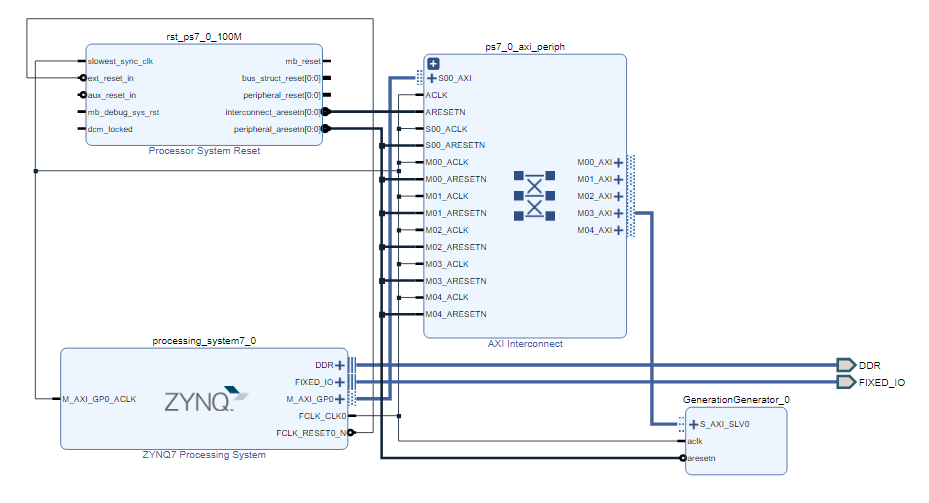
\includegraphics[width=0.7\linewidth]{../diagrams/vivadoDesign}}
	\caption{The block design in Vivado of our IP core, the ZYNQ7 processing system, a AXI interconnect component and a reset controller.}
	\label{fig:vivadodesign}
\end{figure}

Here it can be seen that we did not include all of the wanted IP cores. This was due to the Simulator using too many resources.


\section{Results}\label{sec:results}
\begin{framed}
6. Implement and test a part of your system using the ZYBO platform including at least one IP core written and verified with the HLS tool.
\end{framed}

This section shows and elaborates on the results in performance and utilization of all the designs we purposed in section \ref{sec:archdesign}. This includes a high-level synthesis report of the two IP cores (GenerationGenerator and Simulator) and the user application, that was implemented in C++ and deployed to the ZYBO board with the use of OSAPI threads and FreeRTOS. Overall, our results show that simple fixed-point arithmetic can be accelerated in an hardware FPGA at relative low cost, however more complicated floating point computations are better done in software, as the number of required DSP's and lookup tables rapidly increase in such cases.

\subsection{HLS of the GenerationGenerator core}

The IP core was synthesized in C using a VivadoSimulator, a period of 20 and Verilog as the RTL language. Target device is a Zybo model xc7z010clg400-1. We used a SystemC stimuli file to invoke the IP core, which can be found in Appendix A. Figure \ref{fig:ggperformanceestimates} shows the performance estimates of the applied design. We seen that the estimated clock is well within our target of 20 with an uncertainty of 2.50 and the latency lie in range of 270 to 271.

\begin{figure}[htbp]
	\centering
	\fbox{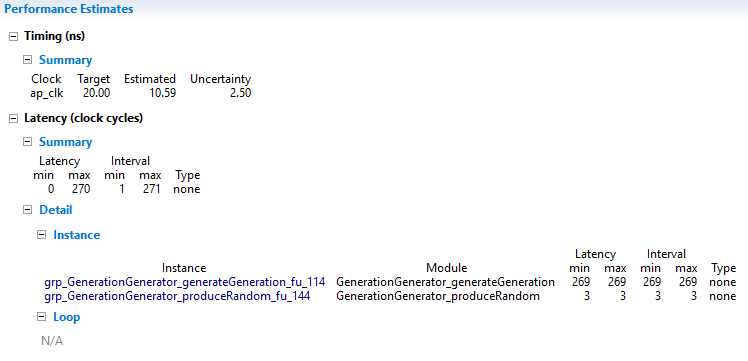
\includegraphics[width=1.0\linewidth]{../diagrams/GGperformanceEstimates.png}}
	\caption{X}
	\label{fig:ggperformanceestimates}
\end{figure}

Figure \ref{fig:ggutilizationestimates} shows utilization of hardware estimates. We see that the demand of resources are well within range of what is available on the Zybo board. 

\begin{figure}[htbp]
	\centering
	\fbox{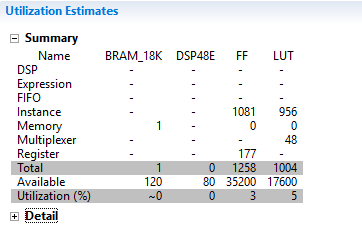
\includegraphics[width=1.0\linewidth]{../diagrams/GGutilizationEstimates.png}}
	\caption{X}
	\label{fig:ggutilizationestimates}
\end{figure}

Figure \ref{fig:gginterface} shows the generated interface signals. These echo the interfaces we defined in the definition of source file. Direction indicate if they are to be read or written to. The bit length stems from the width of a chromosome.

\begin{figure}[htbp]
	\centering
	\fbox{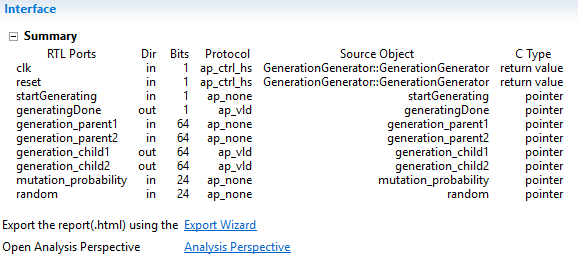
\includegraphics[width=1.0\linewidth]{../diagrams/GGinterface}}
	\caption{}
	\label{fig:gginterface}
\end{figure}

Figure \ref{fig:generationgeneratortrace} shows the trace output after running a simulation with a stimuli. We seen that the random input data changes continually, and when the generating core is started, it uses the two parents and a mutation probability to create new children chromosomes and output these.

\begin{figure}[htbp]
	\centering
	\fbox{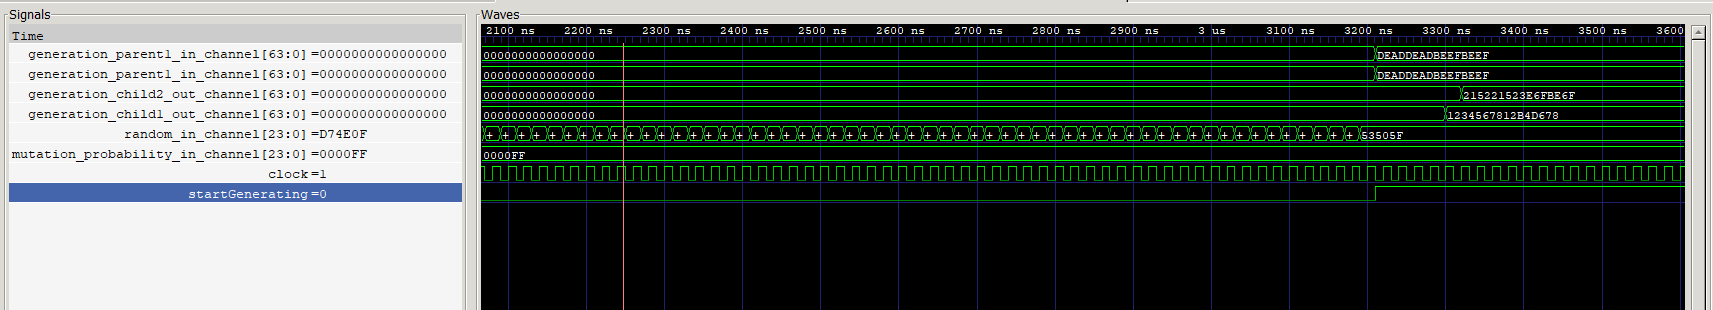
\includegraphics[width=1\linewidth]{../diagrams/GenerationGeneratorSim.png}}
	\caption{A trace diagram that shows all bidirectional signals of the module during a example stimulation.}
	\label{fig:generationgeneratortrace}
\end{figure}

\subsection{HLS of the Simulator core}

The IP was synthesized with the same settings as the GenerationGenertor in the Vivado HLS tool. We used a SystemC stimuli file to make calls to the IP core, which can be found in Appendix A. Figure \ref{fig:simperformanceestimates} shows performance estimates, with the estimated clock being within the range of the target clock and the latency being from  0 to 96. 

\begin{figure}[htbp]
	\centering
	\fbox{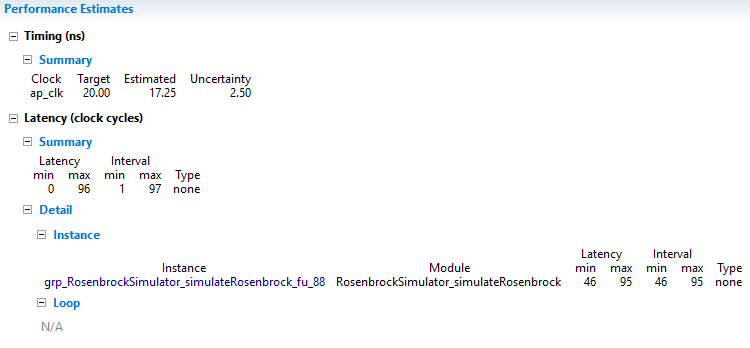
\includegraphics[width=1.0\linewidth]{../diagrams/SimperformanceEstimates.png}}
	\caption{X}
	\label{fig:simperformanceestimates}
\end{figure}

In figure \ref{fig:ggutilizationestimates} we see the utilization estimates of running the simulation in hardware. The total resource demand exceed those of the platform, the Zybo board, by quite a significant margin. The algorithm need 592 DSP48E's, but only 80 are available. Likewise it needs 39988 flip-flops and 22918 lookup tables, but fewer are available. This means that the current implementation will not be runnable on hardware.

\begin{figure}[htbp]
	\centering
	\fbox{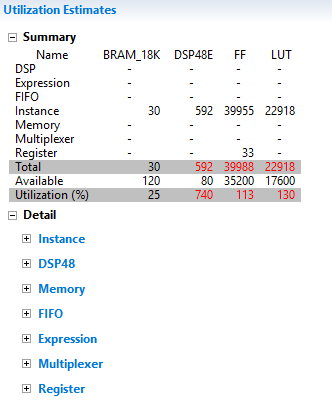
\includegraphics[width=1.0\linewidth]{../diagrams/SimutilizationEstimates.png}}
	\caption{X}
	\label{fig:simutilizationestimates}
\end{figure}
Figure \ref{fig:siminterface} shows the generated interface signals with the RTL ports and their respective direction and bit length. 

\begin{figure}[htbp]
	\centering
	\fbox{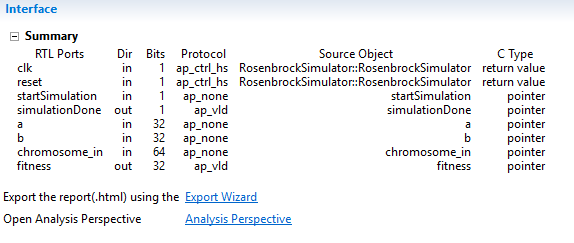
\includegraphics[width=1.0\linewidth]{../diagrams/Siminterface}}
	\caption{X}
	\label{fig:siminterface}
\end{figure}}


%\section{Theory and concepts}
%\section{Modeling in SystemC}
%\section{Simulation results}
\section{Conclusion}
\bibliographystyle{plain}
\bibliography{bibliography}
\end{document}
